\chapter{Návrh riešenia}
Východiskom pre riešenie spracovania akceleračných dát budú nasledujúce výskumné otázky, ktoré
sa pokúsime zodpovedať za kontrolovaných aj reálnych podmienok primárne na vlastných datasetoch:

\section{Požiadavky - Výskumné otázky}
\begin{itemize}[noitemsep]
	\item Ako vplýva nastavenie parametrov metód časovej a frekvenčnej analýzy na úspešnosť detekcie význačných udalostí,
	teda náhlych zmien distribúcie v čase a hlavných frekvenčných komponentov?
	\item Aká úspora v množstve prenášaných dát sa dosiahne rozličnými technikami na sumarizáciu vzoriek?
	\item Aká je výpočtová náročnosť a časť odozvy spôsobov detekcie udalostí?
	\item Aká je presnosť odhadu rýchlosti a polohy z akcelerácie?
	\item Aká syntax pravidiel môže byť vhodná na vzdialenú konfiguráciu dátovej pipeline IoT zariadenia?
	\item Ktorý bezdrôtový komunikačný protokol postačuje pre implementované modely spracovania?
\end{itemize}

Navrhované zariadenie bude postavené na platforme mikrokontroléra ESP32 od Espressif, pretože pri nízkej
obstarávacej cene ponúka možnosť konektivity s Wifi a Bluetooth a v porovnaní s podobnými zariadeniami dostatočný
výpočtový výkon a kapacitu pamätí, čo ho činí vhodný na experimentovanie. Diagram aktivít na obr. \ref{fig:design}
vizualizuje navrhovaný beh činností na zariadení.

Po zapnutí sa začne čítanie vzoriek z akcelerometra s nastaveným dynamickým rozsahom, nad určitú
prahovú úroveň amplitúdy a so vzorkovacou frekvenciou podľa ODR. Podľa pravidlami aktivovanými modulmi bude
súbežne vykonateľných 5 ciest spracovania.

Frekvenčná analýza bude pozostávať z krokov oknovania signálu  zvoliteľnou oknovou funkciou nastaviteľnej veľkosti,
následne sa signál transformuje do frekvenčnej domény,
kde dôjde k vyhladeniu spektra kĺzavým priemerom alebo Welchovou metódou a nakoniec sa podľa prítomnosti špičiek
vo frekvenčnom vedierku vytvorí udalosť na začiatku a na konci súvislého časového pôsobenia. Časová analýza
bude detegovať náhle zmeny v priebehu signálu na základe štatistík polohy, rozptýlenosti a tvaru
distribúcie vzhľadom na predošlé okná. Okrem toho sa môžu po podvzorkovaní odosielať alebo ukladať ,,surové dáta''
hodnôt veličiny v čase alebo frekvenčných vedierok. Numerická kvadratúra korigovaná obálkami umožní extrahovať zo
snímaného zrýchlenia odhad o rýchlosti a polohe.

\section{Hardvér}
OpenLog VCC zapojený cez MOSFET tranzistor cez BTS117
\begin{figure}[h]
	\centering
	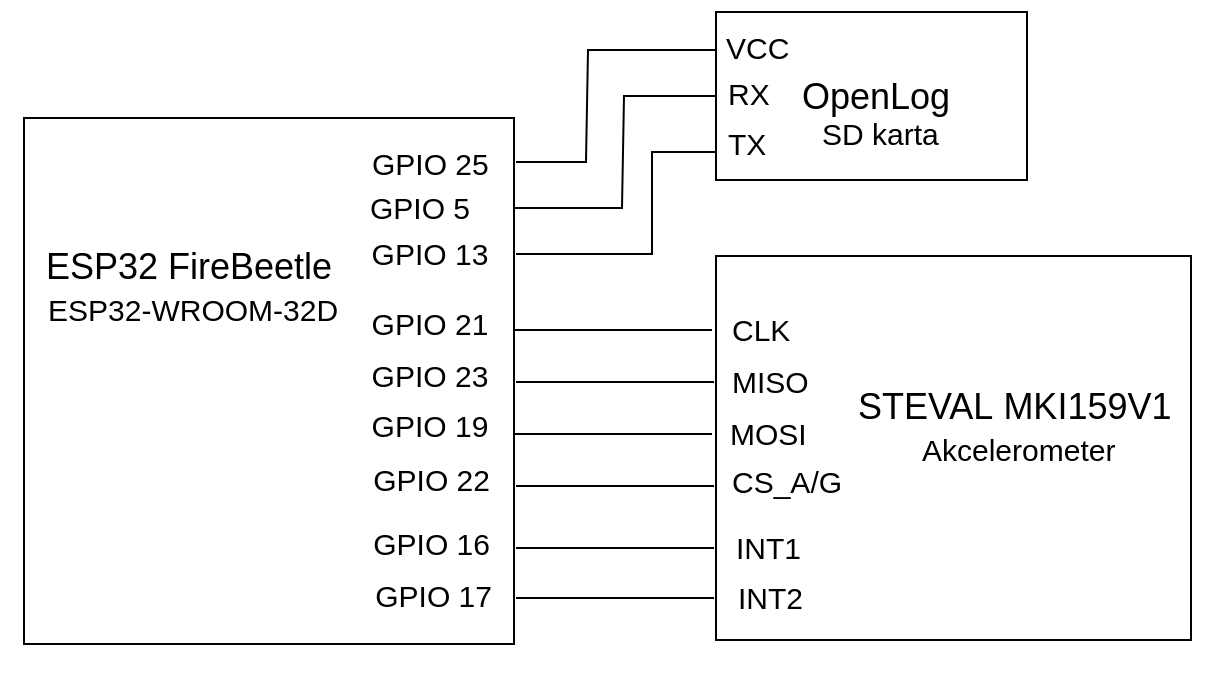
\includegraphics[width=0.8\textwidth]{figures/design/block-circuit-diagram.png}
	\caption{Blokový diagram hardvéru}
\end{figure}

\begin{figure}[h]
	\centering
	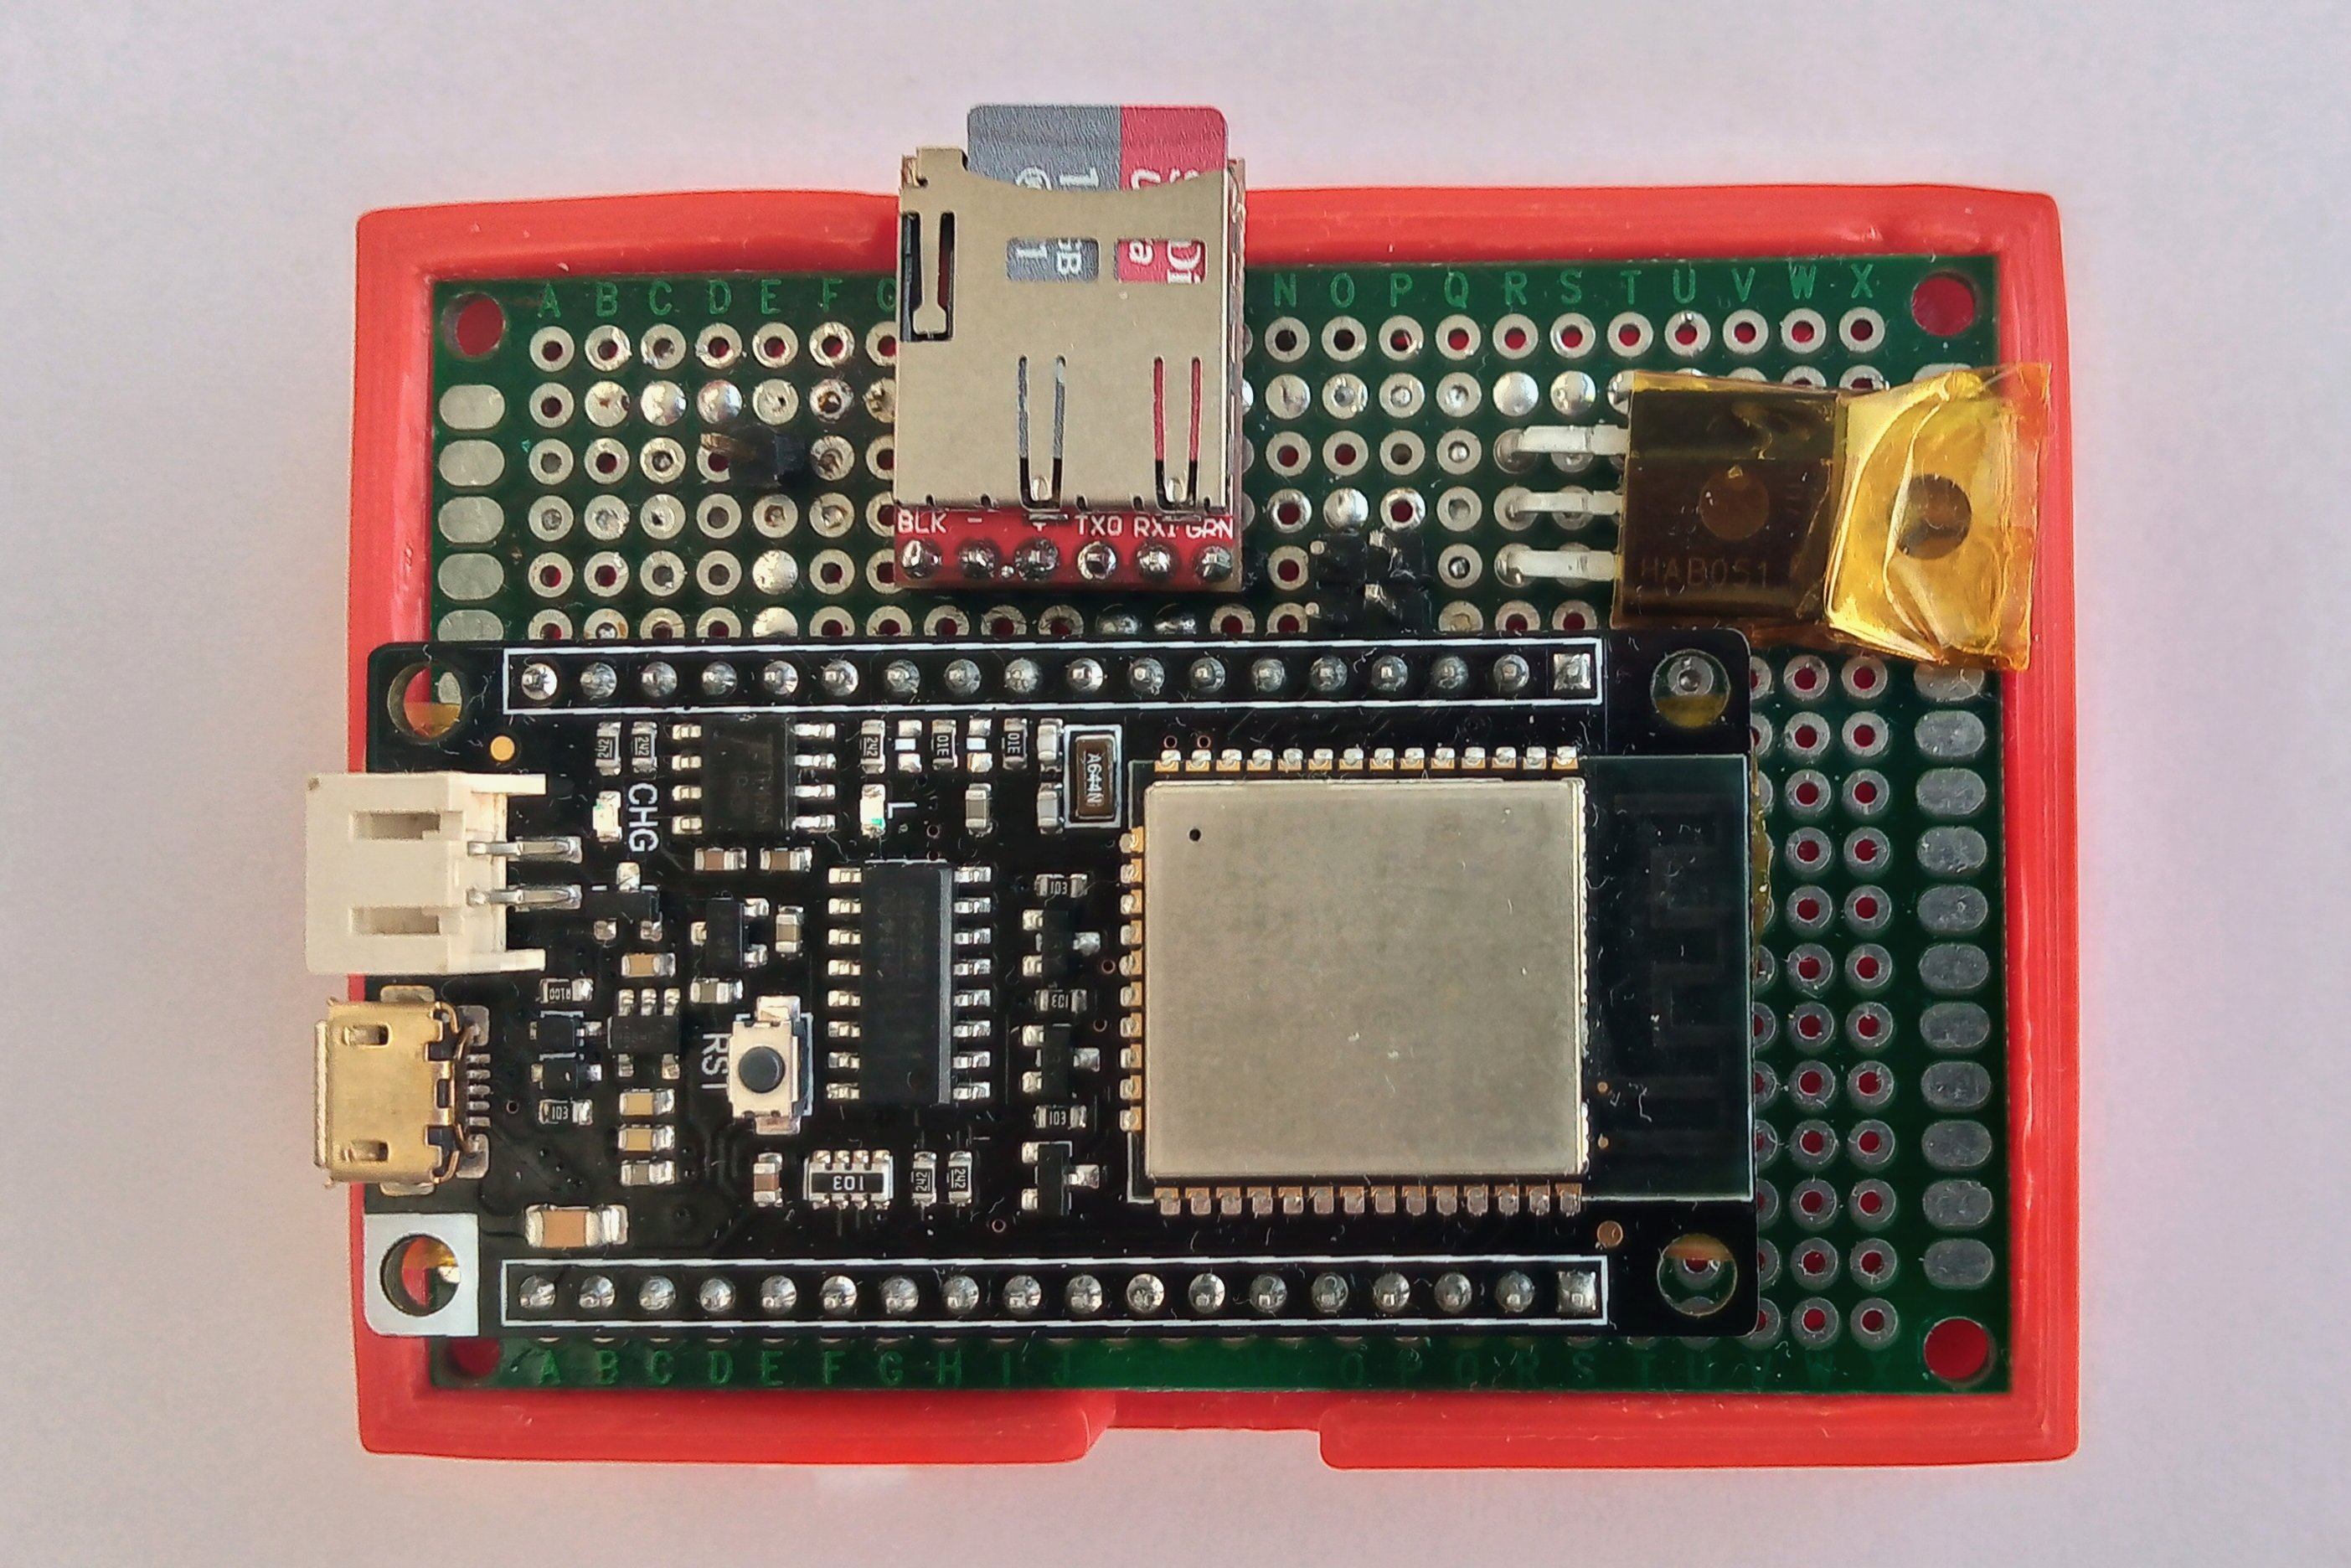
\includegraphics[width=0.7\textwidth]{figures/design/esp32.jpg}
	\caption{Zariadenie}
\end{figure}

\section{Komponenty spracovania signálu}
\begin{figure}[h]
	\centering
	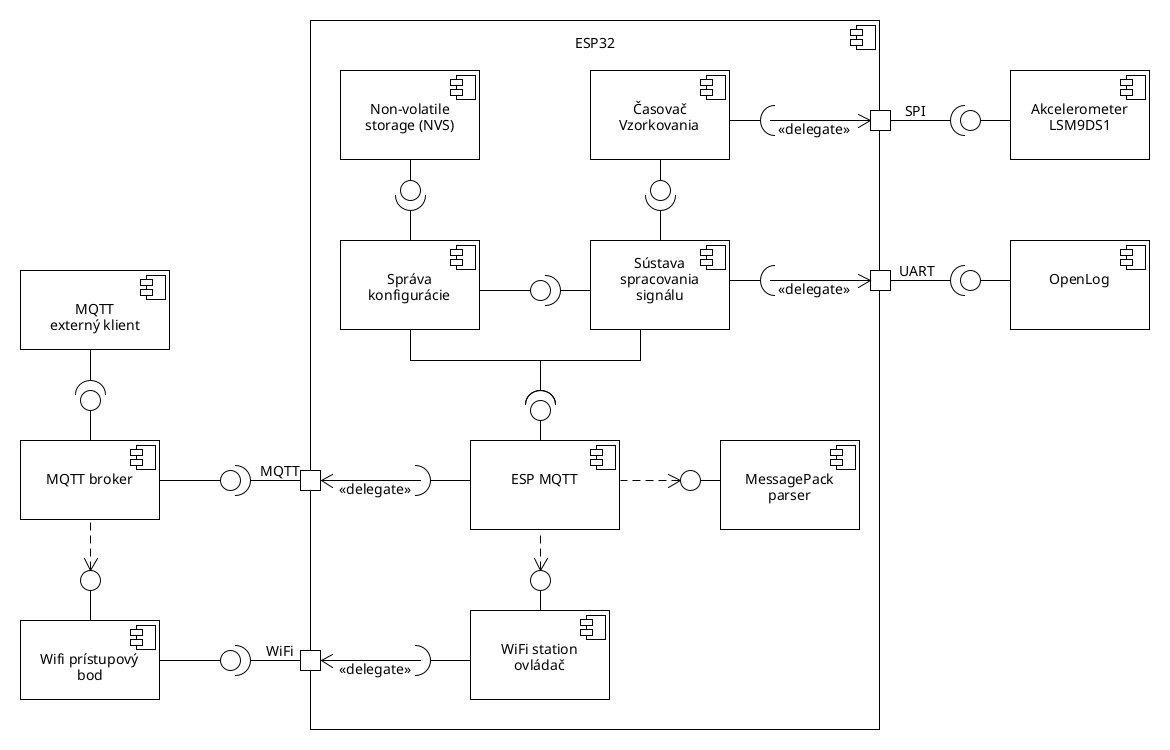
\includegraphics[width=\textwidth]{figures/design/components.png}
	\caption{Diagram komponentov}
\end{figure}

\begin{figure}[h]
	\centering
	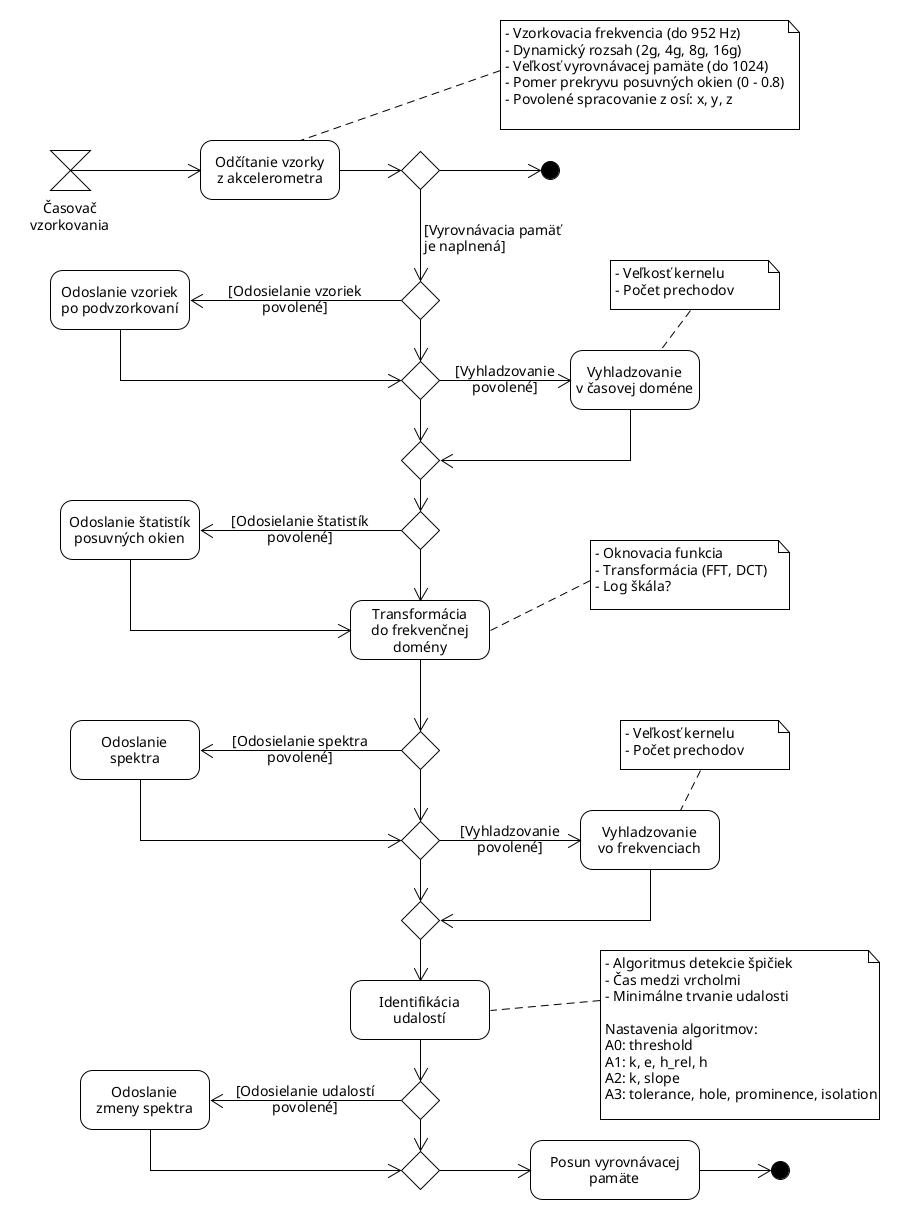
\includegraphics[width=\textwidth]{figures/design/pipeline.png}
	\caption{Diagram aktivít navrhovaného systému na spracovanie dát zo senzora}
\end{figure}

\begin{figure}[h]
	\centering
	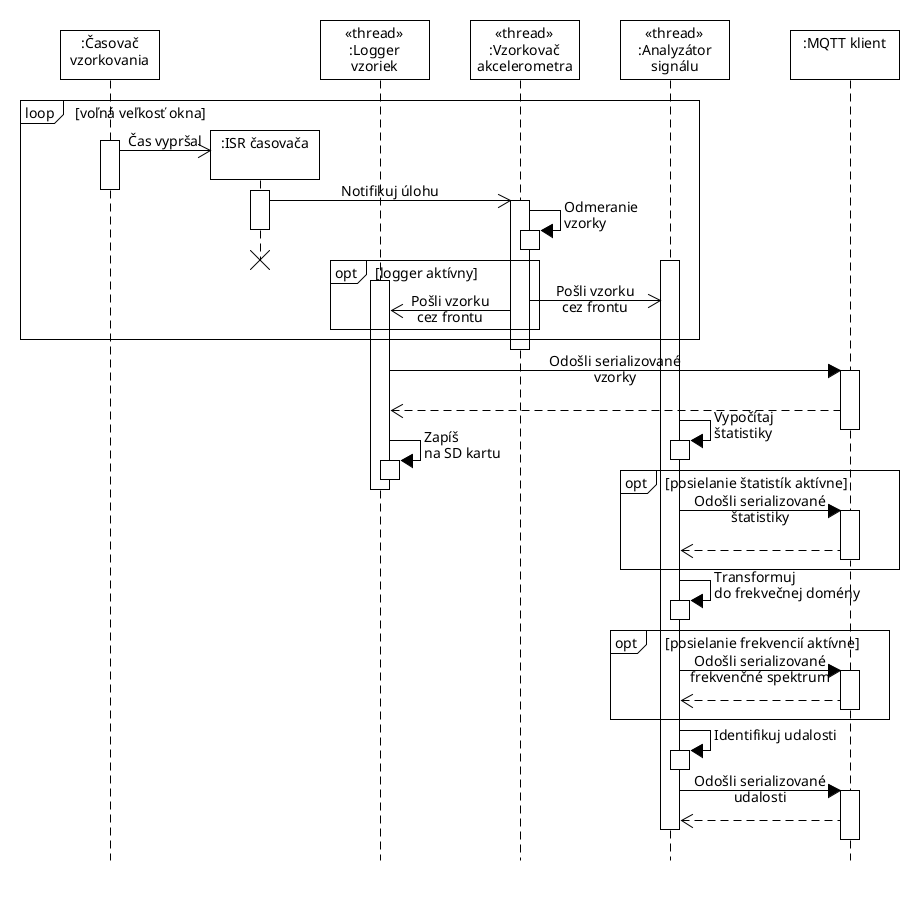
\includegraphics[width=\textwidth]{figures/design/tasks.png}
	\caption{Sekvenčný diagram}
\end{figure}

\begin{figure}[h]
	\centering
	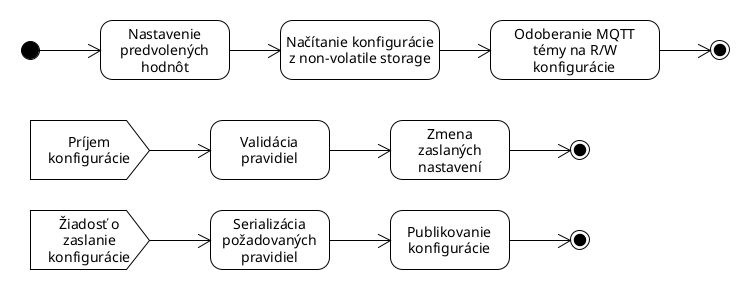
\includegraphics[width=\textwidth]{figures/design/configuration.png}
	\caption{Diagram aktivít konfigurácie}
\end{figure}

\section{Prúdový algoritmus na detekciu zmien zložiek frekvenčného spektra}
Nevidí celý prúd naraz ani ho nemôže celý uložiť. Welchove priemerovanie vyžaduje veľa pamäte pre dlhšie okno.
Ale musíme dosiahnuť odšumenie detegovanie špičiek a zároveň posielať cez sieť menej ako nespracované
frekvenčné vedierka. Detegovanie anomálií, resp. automatické upozornenie na prevládajúce zložky.

\begin{figure}[h]
\centering
\begin{subfigure}[b]{0.8\textwidth}
    \centering
    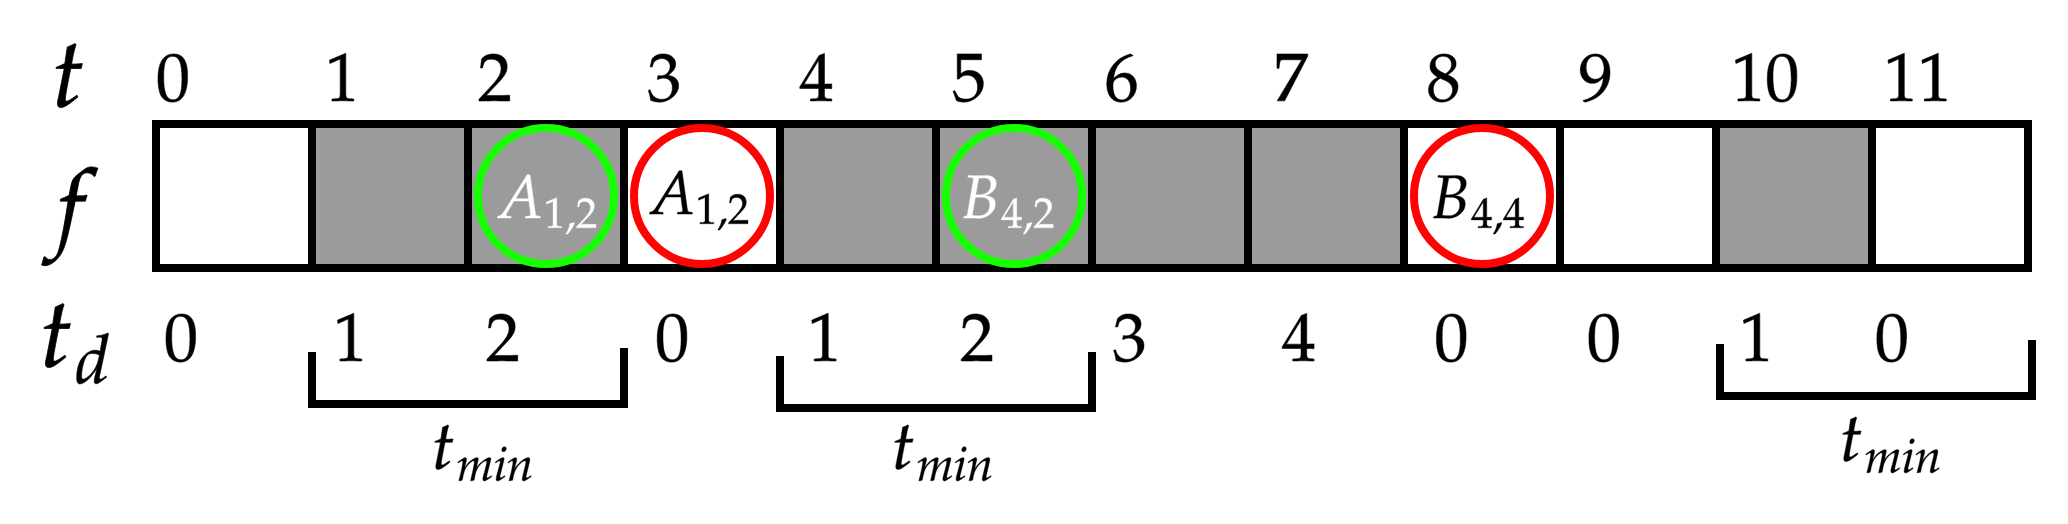
\includegraphics[width=\textwidth]{figures/design/event-detection-min-duration.png}
    \caption{Minimálne trvanie udalosti $t_{\min} = 2$}
\end{subfigure}
\begin{subfigure}[b]{0.8\textwidth}
    \centering
    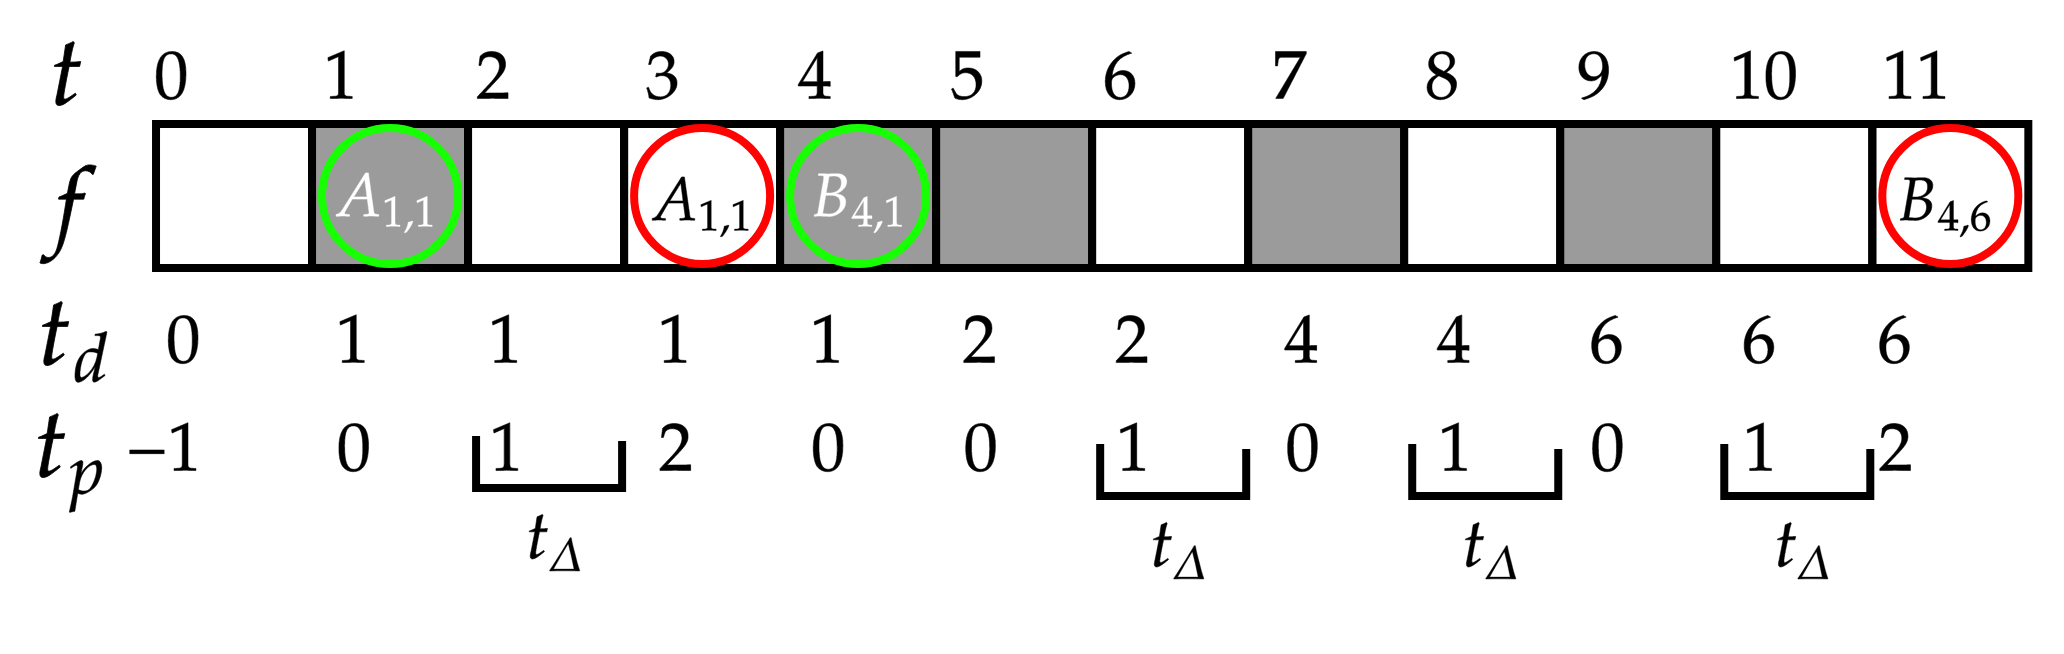
\includegraphics[width=\textwidth]{figures/design/event-detection-time-proximity.png}
    \caption{Maximálna vzdialenosť špičiek $t_{\Delta} = 1$ v čase}
\end{subfigure}
\caption{Parametre algoritmu na detekciu udalostí. $t$ je poradové číslo okna, $f$ je stav detegovanie špičky
vo frekvenčnom vedierku, $t_d$ je trvanie udalosti (duration), $t_p$ je počet okien do minulosti naposledy videnej špičky (past)}
\end{figure}

\begin{algorithm}[h]
\caption{Detektor zmeny frekvenčnej zložky}
\begin{algorithmic}[1]
\Require{$event$, $bin$, $t$, $t_{min}$, $t_{\Delta}$}
\If {V predošlom okne $t - 1$ bola emitovaná udalosť Koniec}
	\State Vynuluj udalosť: $event$: $duration \gets amplitude \gets 0$, $lastSeen \gets -1$
\EndIf

\If {$\mathrm{IsPeak}(bin)$}  
	\State $link \gets \max\{1, event.lastSeen + 1\}$
	\If {$event.duration < t_{min} \leq event.duration + link$}
		\State $event.start \gets t - event.duration - link + 1$
		\State \textbf{Emituj udalosť Štart} výskytu frekvencie podľa $event$
	\EndIf
	
	\State \textbf{Inkrementuj} $event.duration$ \textbf{o} $link$
	\State \textbf{Inkrementuj} $event.amplitude$ \textbf{o} $(bin - event.amplitude)\;/\;event.duration$
	\State $event.lastSeen \gets 0$

\ElsIf {$event.lastSeen \geq 0$}
	\State \textbf{Inkrementuj} $event.lastSeen$ \textbf{o}  $1$

	\If {$events.lastSeen > t_{\Delta}$}
        	\If {$event.duration \geq t_{min}$}
        		\State \textbf{Emituj udalosť Koniec} výskytu frekvencie podľa $event$
        	\EndIf
        \Else
        	\State Vynuluj udalosť: $event$: $duration \gets amplitude \gets 0$, $lastSeen \gets -1$
        \EndIf
\EndIf
\end{algorithmic}
\label{algo:event-detector}
\end{algorithm}

\section{Generátor signálov}
\begin{figure}[h]
   \centering
    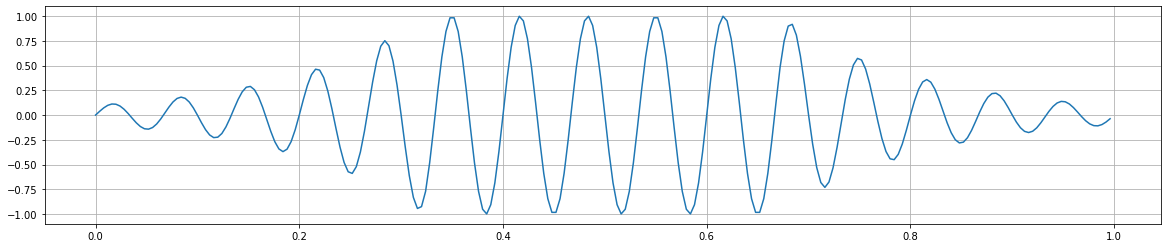
\includegraphics[width=0.8\textwidth]{figures/verification/fade-in-sinusoid.png}
   \caption{Základný tón formujúci syntetický signál}
\end{figure} 



